% Created 2024-09-13 Fri 20:22
% Intended LaTeX compiler: pdflatex
\documentclass[letterpaper, 12pt]{article}
\usepackage[utf8]{inputenc}
\usepackage[T1]{fontenc}
\usepackage{graphicx}
\usepackage{longtable}
\usepackage{wrapfig}
\usepackage{rotating}
\usepackage[normalem]{ulem}
\usepackage{amsmath}
\usepackage{amssymb}
\usepackage{capt-of}
\usepackage{hyperref}
\usepackage{minted}
\usepackage{xcolor}
\usepackage{hyperref}
\usepackage{tocloft}
\usepackage{minted}
\usemintedstyle{manni}
\usepackage{pdfpages}
\usepackage{fancyhdr}
\usepackage{graphicx}
\usepackage[top=1.4in, left=0.5in, right=0.5in, bottom=0.8in]{geometry}
\usepackage[T1]{fontenc}
\usepackage{helvet}
\pagestyle{fancy}
\renewcommand{\headrulewidth}{0pt}
\renewcommand{\footrulewidth}{0pt}
\setlength{\parindent}{0em}
\setlength{\parskip}{1em}
\usepackage{hyperref}
\usepackage {color}
\usepackage {tabularray}
\usepackage{xcolor}
\hypersetup{
colorlinks=true,
linkcolor=blue,
filecolor=magenta,
urlcolor=cyan,
citecolor=green,
pdfborder={0 0 0}
}
\usepackage[most]{tcolorbox}
\author{Hilduara Abreu}
\date{2024-09-05}
\title{School Year 2024-25 | Principal Message June 2024}
\hypersetup{
 pdfauthor={Hilduara Abreu},
 pdftitle={School Year 2024-25 | Principal Message June 2024},
 pdfkeywords={},
 pdfsubject={},
 pdfcreator={Emacs 29.4 (Org mode 9.6.15)}, 
 pdflang={English}}
\begin{document}

\fancyfoot[C]{\setlength{\unitlength}{1in}\begin{picture}(5,0)\put(-1.8,-0.5){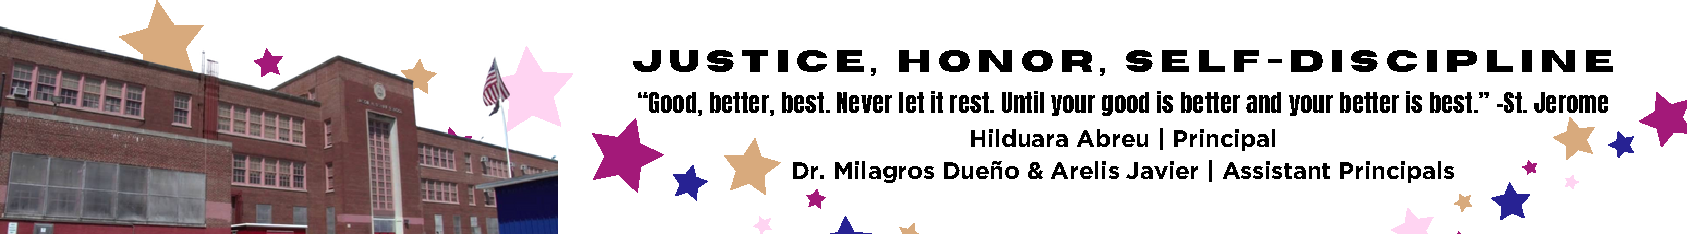
\includegraphics[width=8.8in,height=1.3in]{logo-1}}\end{picture}}
\fancyhead[C]{\setlength{\unitlength}{1in}\begin{picture}(5,0)\put(-1.9,-0.5){
\includegraphics[width=8.9in,height=1.3in]{logo-2}}\end{picture}}
\fancyhead[R]{\thepage}
\pagenumbering{gobble}

\begin{document}
\newpage
\vspace*{-0.5cm}
\textbf{Subject: Welcome to June, 2024 at PS 192: The School of Joyful Learning}!

Greetings Parents and Guardians,

As we approach the end of this school year, I am filled with immense pride for the achievements we have made together at P.S. 192 and am equally excited about the plans we have for the upcoming school year.

I extend my heartfelt gratitude to all parents who have contributed to our school events throughout the year. Your dedication in organizing and participating in our activities and your steadfast attendance at our parent workshops have been invaluable. Your unwavering support has made a significant impact on our school community.

Please note that Wednesday, June 26, 2024, will be our Graduation Day and the final day of school. On this day, your children will receive their report cards.

In closing, I would like to wish our fifth-grade students the very best as they transition to Middle School. I will miss each of you and your families and hope you carry with you cherished memories of your time at P.S. 192.

I wish everyone a delightful and restful summer and look forward to collaborating with many of you in the upcoming year.

With Justice, Honor, and Self-Discipline,


\includegraphics[width=0.2\textwidth]{hil_signature}

\textbf{Hilduara Abreu, Principal}

\textbf{The school of Joyful Learning!}

\href{www.ps192.org}{www.ps192.org}
\end{document}
